%%%%%% CMB-S4 Simulations and Data Analysis Chapter, Data Simulation Section  %%%%%%%%%%%%%%%%
 
\section{Data Simulation}

The data simulation subset of the CMB simulation pipeline (Figure \ref{fig_ds}) takes the sky model and applies the mission model to it to generate a simulated data set for that mission. The mission model consists of two parts; the instrument model defines the data acquisition system (telescope, detectors, read-out), while the observation model defines its deployment (scanning strategy, environment). Depending on the degree of detail of the sky, instrument and observation model that we include, the resulting data set can be in any of the data domains - time-ordered (raw or clean), map, or spectral. Inevitably there is a trade-off between the realism of the simulation and the complexity and cost both of generating the model inputs and of performing the simulation, with the choice reflecting both the requirements of the subsequent analyses of the data set and the availability of computational resources.

\begin{figure}[htbp]
\centering
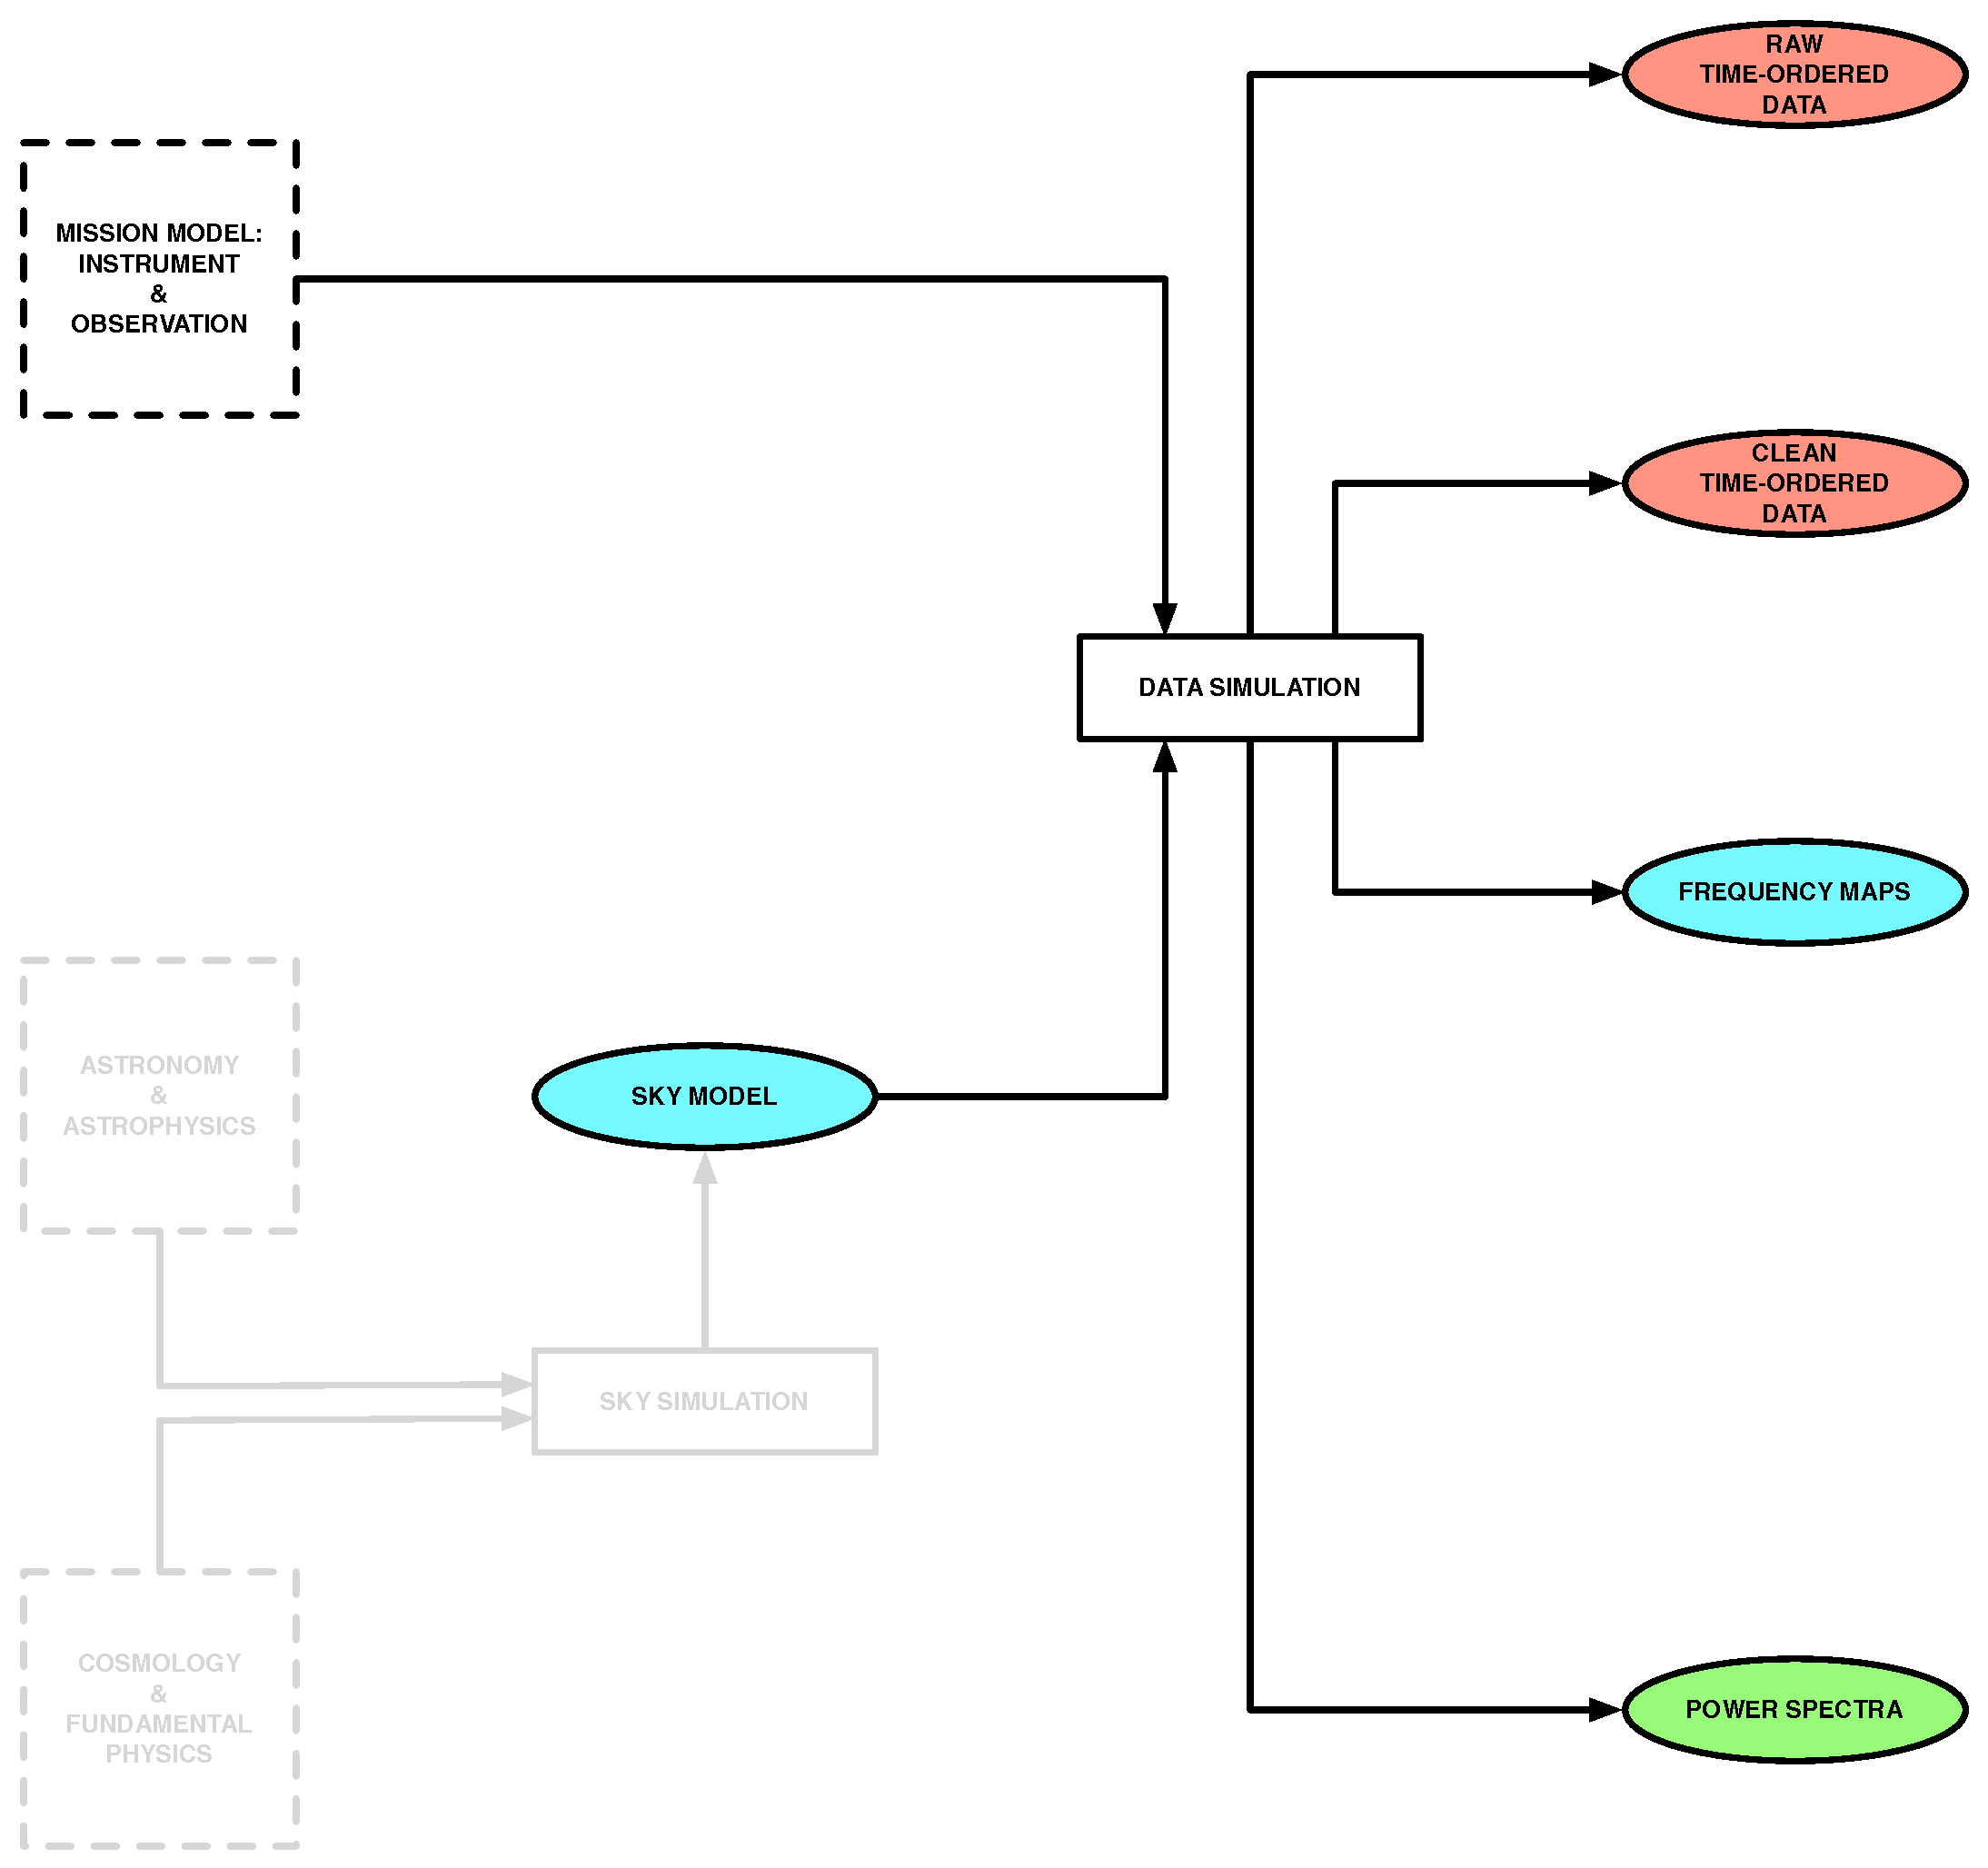
\includegraphics[width=0.5\textwidth]{Analysis/ds}
\caption{The data simulation subset of the CMB simulation pipeline}
\label{fig_ds}
\end{figure}

At the most detailed level, the observation model includes the telescope pointing (typically sampled more sparsely that the detectors), and its environment (comprising the atmosphere and surroundings for a ground-based telescope). Correspondingly, the instrument model includes each detector's polarized $4 \pi$-beam and bandpass (defining the optical power incident on the detector for a given pointing), and a model of its electronics and readout (defining the recorded output data resulting from that optical power).

\subsection{Time Domain}

TOD simulations are necesserily the most expensive to perform, but provide the most precise representation of the mission data. In particular they enable the injection of the full range of systematic effects into the data to assess strategies for their mitigation and to quantify any residuals. As such they are critical for the quantification of uncertainties due to inherently temporal data components such as noise. The TOD simulation is separated into signal and noise components, which are then added prior to the reduction of the total TOD.

For the signal simulation for a given detector, we first apply the detector's bandpass to the sky model, component by component, to build up the total sky for that detector. We then reconstruct the detector pointing from the overall telescope pointing model and generate the astrophysical sky signal for each pointing by convolving the sky model map with the $4 \pi$ beam. The astrophysical sky signal is added to additional simulated signals from atmospheric signal fluctuations and ground pickup (both of which will obviously induce correlated signals across the detectors), and the total signal is propagated through a simple model of the optics to include the polarization angle rotations and optical efficiencies of the optical stages. This results in the total millimeter-wave power incident on the detector. For simulating the clean TOD this is sufficient. However, for the raw TOD we now need to apply a physical model of the detector system and associated readout to convert the optical power into detector output. The details of the physical model depend on the detector technology, but as an example we consider a transition-edge superconducting (TES) bolometer read out with a multiplexed SQUID amplifier. The simulation would then need to model the flow of heat in the TES absorber and the flow of current and magnetic flux through the SQUID readout. Variations in ambient magnetic field could also be added at this stage. Such a simulation would also need to incorporate detector-detector correlations induced by crosstalk or thermal fluctuations.  Additional filters applied by the readout electronics would also be included, including digitization with an analog to digital converter. For MKID or coherent receivers, the physical model would be different in detail, but would include a similarly detailed model.

For the noise simulation we can simply generate a white noise timestream and convolve it with the detector's noise power spectral density (PSD), given in either analytic or numerical form. Cross-correlated noise can be included by simulating multiple noise timestreams each with their own PSD, with some being common to multiple detectors, while piecewise stationary noise simply requires us to use the appropriate PSD for each stationary interval.

\subsection{Map Domain}

Apply symmetric beam in harmonic space, or effective beam (built up over pointings), to bandpassed map.

Use hitmap or 3x3 white noise covariance matrix (built up over pointings) to generate noise map.

\subsection{Spectral Domain}

Model residuals (noise, systematics, component separation, etc) in spectral domain.

%\bibliography{cmbs4}

%%
%% Populate the .bib file with entries from SPIRES Bibtex (preferred)
%% or ADS Bibtex (if no SPIRES entry).
%%  SPIRES will also supply the CITATION line information; please include it.
%%


